\section{Auswertung}
\label{sec:Auswertung}
Jegliche Fehlerrechnung wurde mit der Python-Bibliothek uncertainties \cite{uncertainties} absolviert. Trotz dessen sind die Formeln für
die Unsicherheiten in den jeweiligen Abschnitten angegeben. Allgemeine Rechnungen wurden mit der Python-Bilbiothek numpy \cite{numpy} automatisiert.
\subsection{Kennlinenschar einer Hochvakuumdiode}
\begin{figure}
    \centering
    \caption{Kennlinienschar bei verschiedenen Heizleistungen}
    \label{fig:charcurve}
    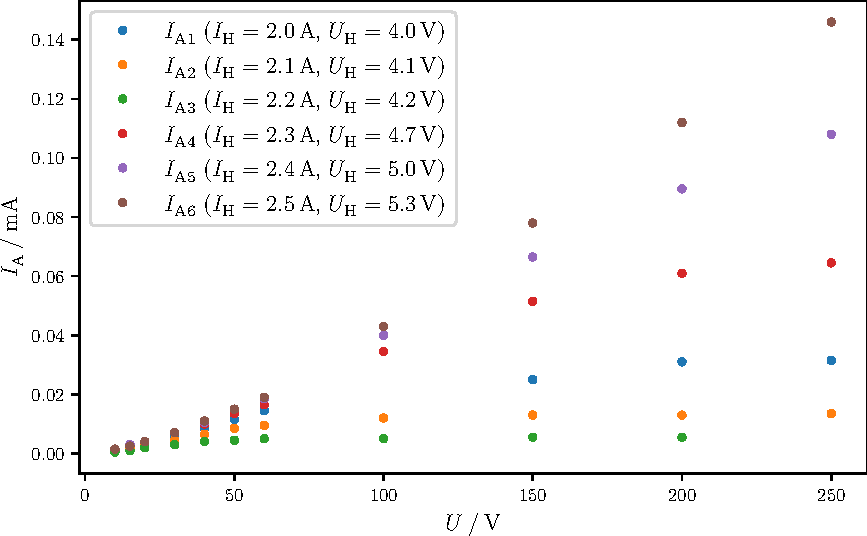
\includegraphics[width = \textwidth]{build/charcurve.pdf}
\end{figure}
In der Abbildung \ref{fig:charcurve} sind die Messwerte  der Absaugströme $I_{\text{A}1}$ bis $I_{\text{A}6}$ bei  6 verschiedenen Heizströmen ($I_\text{H}$)
bzw. -spannungen aufgetragen ($U_\text{H}$). 
Anhand der Graphik können die Sättigungsströme $I_\text{S}$für die Kennlinien von $I_{\text{A}1}$ bis $I_{\text{A}4}$ abgelesen werden.
Diese betragen in etwaa
\begin{align*}
I_{\text{S}1} & = \SI{2.2}{\milli\ampere}   \\
I_{\text{S}2} & = \SI{5.4}{\milli\ampere}   \\
I_{\text{S}3} & = \SI{12.6}{\milli\ampere}  \\
I_{\text{S}4} & = \SI{25.8}{\milli\ampere}  \\
\end{align*}
\subsection{Bestimmung des Raumladungsgebietes}
\begin{figure}
    \centering
    \caption{Regression zur Bestimmung des Raumladungsgebietes}
    \label{fig:exponent}
    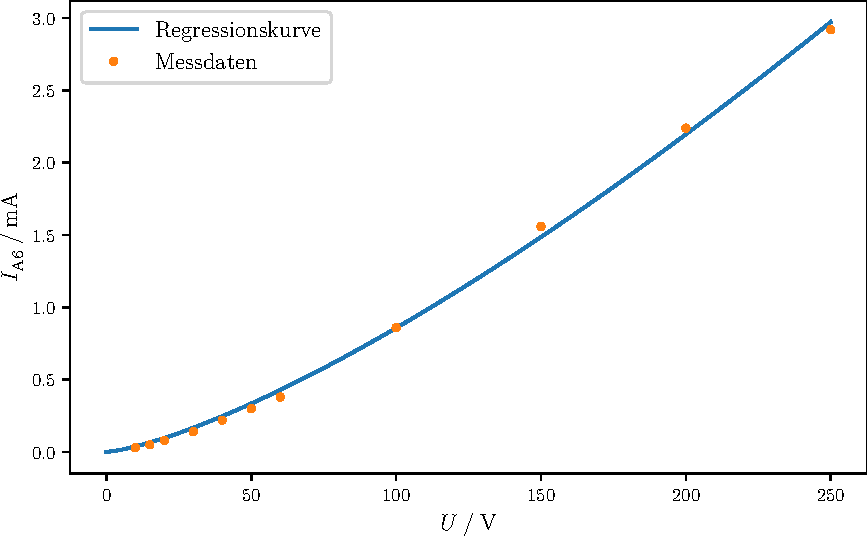
\includegraphics[width = \textwidth]{build/exponent.pdf}
\end{figure}